\chapter{项目部署方案}
 饿了吧得到部署采用前端项目部署在 web 服务器中,后端项目部署在应用服务器中的方案


\section{前端部署}
前端项目部署在 web 服务器中的好处有:
 \begin{itemize}
     \item 可以实现反向代理,提高网站的安全性
     \item 方便维护,一些小的修改不必同时协调前后端开发人员
     \item 对静态资源的加载速度更快
 \end{itemize}
下载nginx
前端端项目根目录执行 npm run build
\begin{figure}[H]
    \centering
    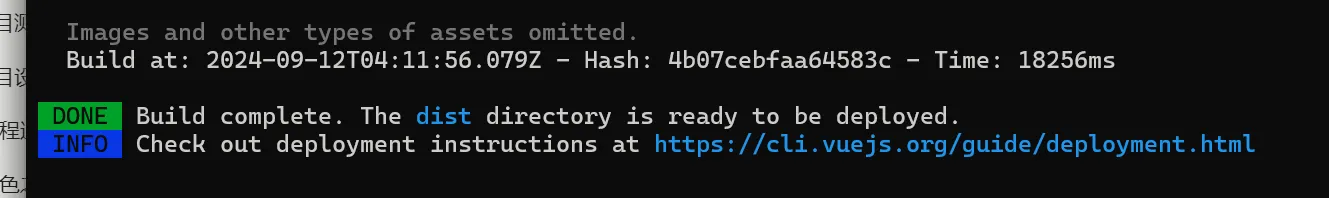
\includegraphics[width=1\linewidth]{pics/部署1.png}
    % \caption{Enter Caption}
    \label{fig:bs1}
\end{figure}
项目的 dist 文件夹下将出现我们打包好的内容并复制到nginx的html文件夹内
\begin{figure}[H]
    \centering
    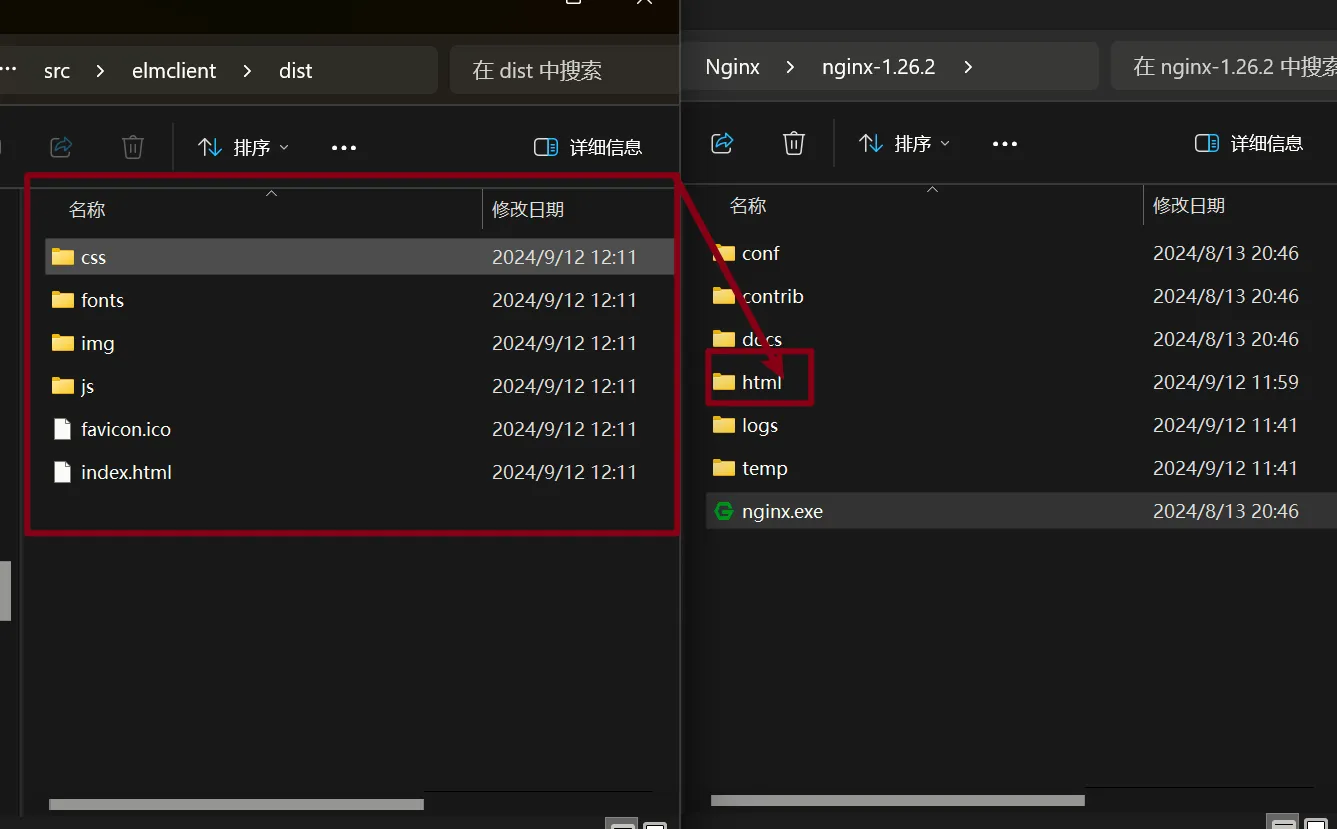
\includegraphics[width=1\linewidth]{pics/部署2.png}
\end{figure}
着,配置一下服务器的默认端口,打开 nginx/conf/nginx.conf,找到 server 的配置处,把 listen 80 改为 listen 8081
\begin{figure}[H]
    \centering
    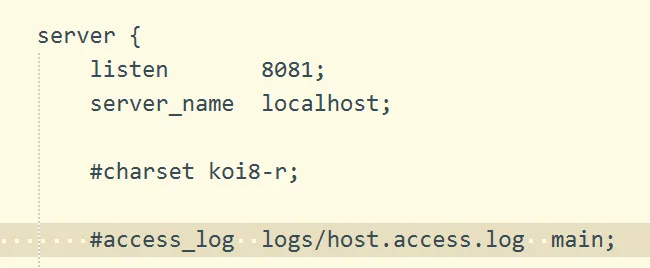
\includegraphics[width=0.5\linewidth]{pics/部署3.png}
\end{figure}
配置完成后,运行 nginx 根目录下的 nginx.exe 即可.
在浏览器访问 http://localhost:8081,即可正常跳转到饿了吧首页.
\section{后端部署}

首先修改后端pom.xml,添加字段:
\begin{figure}[H]
    \centering
    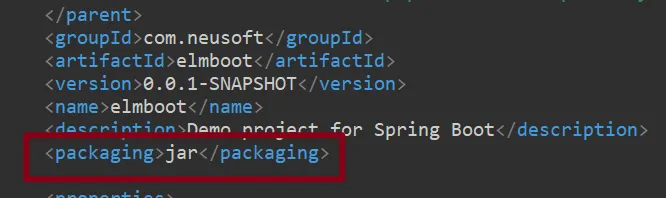
\includegraphics[width=0.8\linewidth]{pics/部署4.png}
\end{figure}
后端根目录运行mvn clean install
\begin{figure}[H]
    \centering
    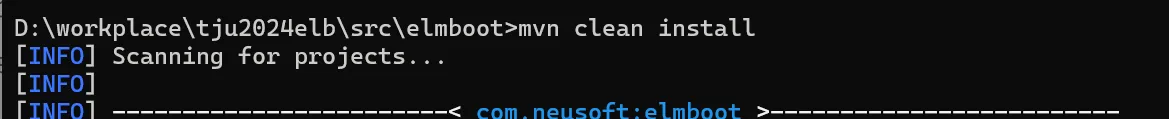
\includegraphics[width=1\linewidth]{pics/部署5.png}
\end{figure}
target目录下生成了jar包
\begin{figure}[H]
    \centering
    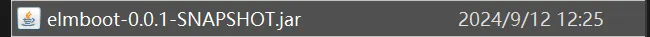
\includegraphics[width=1\linewidth]{pics/部署6.png}
\end{figure}
控制台执行 java -jar elmboot-0.0.1-SNAPSHOT.jar
\begin{figure}[H]
    \centering
    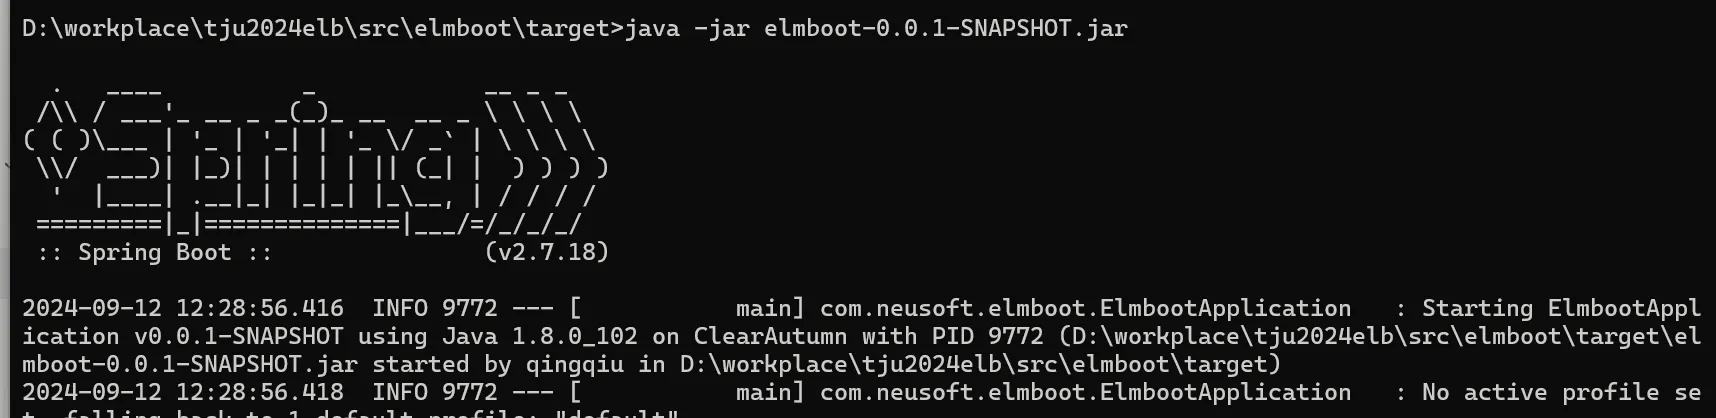
\includegraphics[width=0.8\linewidth]{pics/部署7.png}
\end{figure}
于是后端运行,此时网页即可正常访问后端服务器.